\documentclass[10pt,journal,final]{IEEEtran}% IEEE论文格式
\usepackage{ctex} %中文包
\usepackage{cite} %引用bib文件包
\usepackage{authblk} %maketitle包
\usepackage{setspace} %行距包(vspace)
\usepackage{titlesec} %自定义多级标题格式的宏包
\usepackage{amssymb} %黑板粗体包
\usepackage{boondox-cal} %花体小写字母包
\usepackage[mathscr]{euscript} %用于复高斯分布CN的花体的奇奇怪怪的宏包
\usepackage{amsmath} %数学等式 begin{align}包
\usepackage{graphicx}
\usepackage{epstopdf} %这行和上一行是插入图片要用的基本的宏包
\usepackage{float} %这行是为了强制指定图片位置[H]
\usepackage{caption} %这行是为了取消图片自动编号
\titleformat{\section}[block]{\large\centering}{\uppercase\expandafter{\romannumeral\arabic{section} .}}{0.05em}{ }[]%这行是定义“section”命令的格式
\titleformat{\subsection}[block]{\fontsize{11pt}{20pt}\mdseries\it}{\Alph{subsection}.}{0.05em}{}[]%fontsize{10pt}{20pt}中10pt是字体大小,20pt是行距
\titleformat{\subsubsection}[block]{\normalsize\bfseries\itshape}{\arabic{subsection}-\alph{subsubsection}}{1em}{}[]
\titleformat{\paragraph}[block]{\small\bfseries}{[\arabic{paragraph}]}{1em}{}[]
\title{利用深度学习在时分复用大规模MIMO系统下完成信道感知和混合预编码}
\author[]{Kareem M.Attiah,Foad Sohrabi,and Wei Yu\vspace{-1.2em}}
\affil{Deartment of Electrical and Computer Engineering\vspace{-1.2em}}
\affil{University of Toronto,Toronto,Ontario M55 3G4,Canada\vspace{-1.2em}}%行距1.2
\affil{Emails:$\{$kattiah,fsohrabi,weiyu$\}$@ece.utoronto.ca\vspace{-2.5em}}%行距2.5
\begin{document}
\maketitle
\thispagestyle{empty} 
\pagestyle{empty}
% \noindent 这行代码是取消首行缩进
摘要:本文提出了一种利用深度学习在射频链路数量有限,且运行于时分双工模式下的毫米波大规模多输入多输出系统中完成信道感知、下行链路混合
模拟和数字波束成形的方法。传统的下行链路预编码设计基于两步:第一步通过信道感知矩阵,来接收上行导频,并以此估计高维信道;然后根据检测
到的信道来设计预编码矩阵。可是,这种方法并不总是最佳方法。比如当导频长度很短时,此方法就不是最优方法。本文表明,通过直接从接收的导频
设计模拟感测和下行链路预编码矩阵,而无需中间信道估计步骤,可以显着提高整体系统性能。具体来说,我们提出了一种信道感知和混合预编码方法,
该方法将导频阶段分为模拟阶段和数字训练阶段。在第一阶段利用深度神经网络来设计上行链路信道感知和下行链路模拟波束形成器。随后,我们调整
模拟波束形成器,并基于等效低维信道,设计数字预编码器。本文提出的深度学习架构的一个关键特点是:它分解为独立并行的单用户深度神经网络,
所以可以推广到具有任意用户数的系统。数值比较表明,与基于信道恢复的对应方法相比,本文所提出的方法所需的训练开销明显更少,并且可以利用
相对较少的导频来获得和具有完整信道状态信息的系统一样的性能。% Abstract翻译完毕
\vspace{-0.8em}
\section{介绍}
\vspace{0.1em}
大规模多输入多输出(MIMO)通信由于其出色的抵抗严重路径损耗的能力,已被公认为下一代蜂窝网络中毫米波(mmWave)系统的关键促成因素之一[1]。
大规模MIMO技术在时分双工(TDD)系统中的使用特别吸引人,因为当它的信道互易性与上行链路信道估计结合使用时,MIMO系统中基站(BS)的天线数
量是可扩展的[2]。但是,运用大规模MIMO技术的一个关键问题是由射频(RF)组件带来的高功率消耗和高成本,这使部署常规的全数字波束成形MIMO架
构变得不可行。为了减轻这种硬件限制,在[3],[4]中提出了所谓的混合波束成形架构,其中全数字波束成形器由模拟波束成形器代替,该模拟波束成形
器使用低成本的模拟移相器实现,然后再采用低维数字波束形成器。

即使在理想的信道状态信息(CSI)假设下,混合预编码器的设计通常也是一项艰巨的任务,因为通过移相器阵列实现模拟预编码器会对设计参数施加非凸
的恒定模数约束,这使得优化预编码器的计算量变得非常大。更重要的是,混合架构还严重限制了上行信道的感知能力。然而,大多数当前最新的混合预
编码方案仍遵循将预编码过程分成两个独立步骤的常规通信系统设计方法:(i)信道感测和估计,以及(ii)下行链路预编码设计。在信道估计步骤中,
通常利用毫米波信道的空间相关性[5]-[8]。特别地,由于mmWave信道在角域中具有稀疏表示,所以现有的信道估计方法通常使用压缩感知技术,来基于
例如均方误差度量去恢复信道模型参数。随后,假设估计到的CSI是完美的,BS再构造模拟和数字预编码矩阵[9]–[11]。

本文的主要观察结果是,上述的分离信道估计和混合预编码方法不一定是最佳方法。尤其是当导频序列长度不足以确保CSI准确恢复时,该方法性能不是最
优。在这种情况下,BS处仅可获得CSI的噪声估计,并且现有的预编码方法可能无法提供良好的性能。本文的主要贡献在于指出,旨在针对某个任意距离度
量(例如,均方误差)来重构通道的常规两步设计,不一定是设计最大速率的混合预编码器的最佳方案。我们可以绕过信道估计,直接从基带接收到的导频
中设计预编码矩阵,以获得整体系统性能的显著改善。

本文提出使用深度学习方法,来基于接收的导频直接设计信道感知和混合预编码矩阵。但是,由于混合预编码器由模拟和数字组件组成,因此以数据驱动的
方式同时进行直接设计是非常重要的。但是,训练复杂度和缺少对用户数量的通用处理让这个设计变得不现实。在本文中,我们提出了一种替代的基于深度
学习的方案,该方案克服了上述限制,但仍绕过了基于模型的显式信道估计。为此,我们建议将上行链路导频训练分为两个单独的阶段,其中在第一阶段中,
我们采用深度神经网络(DNN),该网络结合了感测矩阵的设计并将基带导频观测结果直接映射到模拟预编码矩阵中。在第二阶段,我们利用观察结果,一
旦确定了模拟波束成形矩阵,就可以将端到端混合预编码系统转换为低维全数字系统,从而设计出数字预编码矩阵。数值模拟表明,尤其是在短导频长度的
情况下,这种方案是有利的,并且相对于基于常规信道恢复的方案而言,可以获得明显更好的性能。

值得注意的是,许多现有工作已经提出在具有混合架构的mmWave大规模MIMO系统中使用DNN来取代关键设计组件,例如用DNN取代信道估计[12],取代具有
完美/不完美CSI的预编码设计[13]–[15],或取代以上两方面[16]。但是,所有这些工作都采用了传统的信道估计和预编码分离方法,并未充分利用DNN的
潜力来设计端到端下行链路预编码系统。
\vspace{-0.8em}
\section{系统模型} %一级标题
\vspace{-0.8em}
\subsection{下行链路传输} %二级标题
我们考虑一种TDD大规模MIMO系统,该系统在逐块衰落且频率平坦mmWave环境中运行,在该环境中,具有$M$个天线和$N_{RF}$个RF链的BS为$K$个单天线
用户提供服务。使用$s\in\mathbb{C} ^{K}$表示要在下行链路中发送给用户的预期信号的集合,第$k$个用户的复基带接收信号由下式给出:
\vspace{-0.8em}
\begin{align}
y_{k}&=\mathbf{h}_{k}^{H} \mathbf{V} \mathbf{s} +n_{k},\nonumber\\ % \nonumber 取消换行标号
&=\mathbf{h}_{k}^{H} \mathbf{v}_{k} s_{k}+\sum_{j \neq  k}^{} \mathbf{h}_{k}^{H} \mathbf{v}_{j} s_{j}+n_{k}, % &用来换行
\end{align}
其中$\mathbf{V}=[\mathbf{v}_{1},.\,.\,.\, ,\mathbf{v}_{K}]\in\mathbb{C} ^{M\times K}$是下行链路预编码矩阵,$\mathbf{h}_{k}\in\mathbb{C} ^{M}$
是从BS到用户$k$的复数下行链路信道增益的向量,而$n_{k}\sim \mathscr{C} \mathscr{N}  $(0,$\sigma^{2}$)是用户$k$处的加性高斯白噪声。
此外,我们假设BS采用的混合波束成形架构具有有限数量的RF链,$N_{RF}$,其中$K \leq  N_{RF} \leq M$。因此,整个预编码矩阵必须采用以下形式:
\begin{align}
\mathbf{V}=\mathbf{V}_{RF}\mathbf{V}_{D},
\end{align}
其中$\mathbf{V}_{D}\in\mathbb{C} ^{N_{RF}\times K}$是低维数字预编码矩阵,$\mathbf{V}_{RF}\in\mathbb{C} ^{M \times N_{RF}}$是移相
器的模拟预编码矩阵,其项满足恒定模数约束,即$[\mathbf{V}_{RF}]_{ij}=e^{\imath \phi_{ij}}$,其中$\imath$是虚数单位。最后,我们通过要
求$\mathbb{E} [\mathbf{s}\mathbf{s} ^{H}]=\mathbf{I} _{K}$和$\|\mathbf{V}\|_{F}^{2}\leq P_{D} $对发射信号施加功率约束。
\vspace{-2.3em}
\subsection[\itshape]{信道模型}
\vspace{0.005em}
我们考虑散射体数量有限的毫米波传播环境。因此,第$k$个用户的信道向量$\mathbf{h}_{k}$遵循由$L_{p}$主导路径组成的稀疏信道模型:
\begin{align}
\mathbf{h}_{k}=\frac{1}{\sqrt{L_{p}}} \sum_{\ell = 1}^{L_{p}}\alpha_{\ell,k}\mathbf{a}_{t}(\theta_{\ell,k}) ,
\end{align}
其中$\alpha_{\ell,k}\sim \mathscr{C} \mathscr{N}(0,1)$是BS和用户$k$之间的第$\ell$条路径的复数增益,$\theta_{\ell,k}$是对应的离开角
(AoD),而在$\mathbf{a}_{t}(\cdot) $是阵列响应向量。假设在BS处有$M$个天线单元组成的均匀线性阵列,我们有:
\begin{align}
\mathbf{a}_{t}(\theta)=\biggl[1,e^{\imath \frac{2\pi}{\lambda}d\sin(\theta )}, .\,.\,.\, ,
e^{\imath \frac{2\pi}{\lambda}d(M-1)\sin(\theta)}\biggr]^{T},
\end{align}
其中,$\lambda $是波长,$d$是天线间隔。
\vspace{-2.0em}
\subsection{上行链路中基于导频的信道感应}
\vspace{0.2em}
我们假设BS没有信道的先验感知,并且必须基于TDD操作中的信道互易性,通过上行链路导频训练来得到CSI的估计(显式或隐式)[17]。为此,我们考虑
由$L$个时间帧组成的上行链路导频训练,其中用户在每个时间帧中重复发送$K$个相互正交的导频序列。由于RF链有数量限制,BS必须使用以下形式的模
拟感测(或组合)矩阵来感测信道:
\begin{align}
\mathbf{W}_{\mathsf{R}\mathsf{F}}^{(\ell)}\in \mathbb{C} ^{N_{RF}\times M},\qquad \ell \in \{1,.\,.\,.\, ,L \},
\end{align}
其一元项必须满足恒模约束$[\mathbf{W}_{\mathsf{R}\mathsf{F}}^{(\ell)}]_{ij}=e^{\imath \psi_{ij}}$。

令$\mathbf{X} \in \mathbb{C} ^{K \times K}$为一元矩阵,其行对应于用户发送的正交导频,则第$\ell $个时间帧在BS处的$N_{\mathsf{R} \mathsf{F} }
\times K$接收信号由下式给出:
\begin{align}
\mathbf{R}^{(\ell)}=\sqrt{P_{\mathsf{U}}}\mathbf{W}_{\mathsf{R}\mathsf{F}}^{(\ell)}\mathbf{H}\mathbf{X} +\mathbf{W}_{\mathsf{R}\mathsf{F}}^{(\ell)}
\mathbf{N}^{(\ell)},\quad \ell \in \{1,.\,.\,.\, ,L\},
\end{align}
其中$\mathbf{H}=[\mathbf{h}_{1},.\,.\,.\, ,\mathbf{h}_{K}]\in \mathbb{C}^{M \times K}$和$\mathbf{N}^{(\ell)}=[\mathbf{n}_{1}^{(\ell)}
,.\,.\,.\, ,\mathbf{n}_{K}^{(\ell)}] \in \mathbb{C}^{M \times K}$是所有用户的信道和噪声矩阵,$P_{\mathbf{U}}$是在单个时间帧内为每个
用户分配的功率。通常$N_{\mathbf{R}\mathbf{F}}\ll M$,因此我们需要多个时间帧(即$L>1$)来捕获用户信道。

由于导频是正交的,因此我们有$\mathbf{X} \mathbf{X}^{H}=\mathbf{I}_{K}$,因此BS可以将接收到的信号乘以$\mathbf{X}^{H}$来获得:
\begin{align}
\tilde{\mathbf{Y}}^{(\ell)}=\sqrt{P_{\mathbf{U}}}\mathbf{W}_{\mathbf{R}\mathbf{F}}^{(\ell)}\mathbf{H}+\mathbf{Z}^{(\ell)},
\ell \in\{1,.\,.\,.\, ,L\},  
\end{align}
其中$\mathbf{Z}^{(\ell)}=\mathbf{W}_{\mathbf{RF}}^{(\ell)}\mathbf{N}^{(\ell)}\mathbf{X}^{H}$是第$\ell$个时间帧中对应的噪声矩阵。
用$\tilde{\mathbf{y}}_{k}^{(\ell)}$表示$\tilde{\mathbf{Y}}^{(\ell)}$的第$k$列,我们可以得到:
\begin{align}
\tilde{\mathbf{y}}_{k}^{(\ell)}=\sqrt{P_{\mathbf{U}}}\mathbf{W}_{\mathbf{R}\mathbf{F}}^{(\ell)}\mathbf{h}_{k}+\mathbf{z}_{k}^{(\ell)},
\ell \in\{1,.\, .\, .\, ,L\}.
\end{align}
通过垂直堆叠$\tilde{\mathbf{y}}_{k}^{(\ell)}$可获得在整个导频传输阶段中,由于第$k$个用户的传输而产生的$N_{\mathbf{RF}}L$接收矢量
(在乘以$\mathbf{X}^{H}$后):
\begin{align}
\tilde{\mathbf{y}}_{k}\triangleq 
\begin{bmatrix}
    \tilde{\mathbf{y}}_{k}^{(1)} \\
    \vdots \\
    \tilde{\mathbf{y}}_{k}^{(L)}
\end{bmatrix}
=\sqrt{P_{\mathbf{U}}} 
\begin{bmatrix}
    \mathbf{W}_{\mathbf{RF}}^{(1)} \\
    \vdots \\
    \mathbf{W}_{\mathbf{RF}}^{(L)}
\end{bmatrix}
\mathbf{h}_{k}+\mathbf{z}_{k}, 
\end{align}
其中$\mathbf{z}_{k} \in \mathbb{C}^{N_{\mathbf{RF}}L}$是相应的噪声矢量。
\vspace{-2.0em}
\subsection{设计目标}
\vspace{0.2em}
现在可以如下说明信道感知和混合预编码问题。假设根据(3)描述的信道模型,我们需要确定感知矩阵$\{\mathbf{W_{RF}}^{(\ell)}\}$,从而可以将
模拟和数字预编码矩阵$\mathbf{V_{RF}}$和$\mathbf{V_{D}}$设计为接收导频信号$\tilde{\mathbf{y}}_{k}$的函数。更具体地说,我们选择下行链
路总速率作为总体目标函数,即
\begin{align}
R=\sum_{k}^{}R_{k},  
\end{align}
其中$R_{k}$是用户$k$可达到的速率,由下式给出:
\begin{align}
R_{k}=\log_{2}\biggl(1+\frac{|\mathbf{h}_{k}^{H}\mathbf{v}_{k}|^{2}}{\sum_{j\neq k} |\mathbf{h}_{k}^{H}\mathbf{v}_{j}|^{2}
+\sigma ^{2}} \biggr)\,.
\end{align}
注意,总速率表达式对感知矩阵$\{\mathbf{W_{RF}}^{(\ell)}\}$的选择的依赖性是隐含的。特别地,从(9)中我们观察到,感知矩阵
$\{\mathbf{W_{RF}}^{(\ell)}\}$的设计至关重要,因为它们起着汇总用户信道信息的重要作用,因此会直接影响我们构造的混合预编码矩阵的质量。
\vspace{-0.3em}
\section{建议的编码方案}
\vspace{-0.3em}
\subsection{动机} 
\vspace{0.2em}
常规的通信系统设计通常依赖于分析方法来分别执行信道估计和预编码设计。在这样的方案中,通常假设一些信道模型。 然后根据一些距离度量来估计
模型参数。 然而,问题在于,这些距离度量可能与使整体系统性能最大化的最终目标不完全匹配。我们认为这种可能的失配是限制传统系统设计的关键,
但是在其他方面是必要的,以确保传统的设计问题是可处理的。现在,数据驱动技术的出现使不同的范例成为可能。不再需要遵守上述分离,即可以完全
绕开CSI估计,并从基带接收的导频直接设计混合预编码器可能更好。换句话说,由于DNN作为通用函数逼近器的强大功能,现在可以实现同时包含信道感
知/估计和混合预编码的端到端设计。更准确地说,设计问题变成了学习感知矩阵$\{\mathbf{W_{RF}}^{(\ell)}\}$以及直接映射下面的矩阵$\mathcal{F} (\cdot )$:
\begin{align}
(\mathbf{V}_{\mathbf{RF}}^{\ast},\mathbf{V}_{\mathbf{D}}^{\ast})=\mathcal{F}(\tilde{\mathbf{y}}_{1},.\,.\,.\, ,\tilde{\mathbf{y}}_{K}),
\end{align}
其中$\tilde{\mathbf{y}}_{k}$是接收到的导频,而$\mathbf{V}_{\mathbf{RF}}^{\ast}$和$\mathbf{V}_{\mathbf{D}}^{\ast}$是速率最大的预编
码矩阵。再次强调,从(9)开始,$\tilde{\mathbf{y}}_{k}$对感知矩阵$\{\mathbf{W_{RF}}^{(\ell)}\}$具有依赖性。

但是,这种方法的复杂性较高。实际上,由于模拟预编码矩阵和数字预编码矩阵之间的乘法交互作用,使得即使在用户数量少的时候,这种DNN的训练也相
当繁琐。此外,我们希望第II-A节中描述的多用户系统能为不同数量的用户提供服务,但是DNN要输出数字预编码矩阵,其输出维数必须等于用户数量。
为了支持这种动态操作,理想方法是基于每个用户设计DNN。为此,我们在下面开发了一种新颖的DNN架构。 所提出的架构与[16]中的架构有些相似,但是
关键的区别在于我们的方法绕过了中间信道估计步骤。
\vspace{-1.8em}
\subsection{混合预编码的学习方法}
\vspace{0.2em}
本文提出的基于学习的方案将模拟预编码矩阵和数字预编码矩阵的设计解耦。具体来说,我们建议将$L$帧的总体导频训练阶段划分为$L_{a}$帧的模拟训
练阶段和$L_{d}$帧的数字训练阶段,且$L=L_{a}+L{d}$。在模拟训练阶段,使用DNN将在最初的$L_{a}$帧中接收到的基带信号直接映射到模拟预编码矩
阵中。在数字训练阶段,模拟波束形成器是固定的,并且基于在剩下的$L_{d}$帧中接收到的导频信号获得数字预编码矩阵。

\textit{\fontsize{11pt}{20pt}1)模拟训练阶段:}我们将在最初的$L_{a}$个时间帧里从第$k$个用户接收到的导频表示为$\tilde{\mathbf{y}}_{k}^{a}
\triangleq \biggl[\left(\tilde{\mathbf{y}}_{k}^{(1)}\right)^{T},.\,.\,.\, ,\left(\tilde{\mathbf{y}}_{k}^{(La)}\right)^{T}\biggr]^{T}$,
然后由(9),我们可以得到:
\begin{align}
\tilde{\mathbf{y}}_{k}^{a}=\sqrt{P_{\mathbf{U}}}\mathbf{W}_{\mathbf{RF}}^{a}\mathbf{h}_{k}+\mathbf{z}_{k}^{a}, 
\end{align}
其中$\mathbf{W}_{\mathbf{RF}}^{a}\triangleq\biggl[\left(\mathbf{W}_{\mathbf{RF}}^{(1)}\right)^{T},.\,.\,.\, ,
\left(\mathbf{W}_{\mathbf{RF}}^{(La)}\right)^{T}\biggr]^{T}$。在模拟训练阶段,我们旨在设计DNN以学习感知矩阵$\mathbf{W}_{\mathbf{RF}}^{a}$
以及从$\{\tilde{\mathbf{y}}_{k}^{a}\}_{k=1}^{K}$(直接)映射到$\mathbf{V_{RF}}$。但是,我们不是将全部DNN用于所有$k$个用户,我们提出
的架构将整个DNN分解为$K$个并行单用户DNN,这些DNN学习感知矩阵$\mathbf{W}_{\mathbf{RF}}^{a}$。还分解为$K$个从$\tilde{\mathbf{y}}_{k}^{a}$到$\mathbf{V_{RF}}$
第$k$列的并行映射$\mathcal{G}^{(k)}(\cdot )$,即
\begin{align}
\mathbf{v}_{\mathbf{RF}}^{(k)}=\mathcal{G}^{(k)}(\tilde{\mathbf{y}}_{k}^{a}),\quad \forall k\in \{1,.\,.\,.\, ,K\}.
\end{align}
本文的想法是模拟预编码矩阵$\mathbf{V_{\mathbf{RF}}}$由$K$个用户中每个用户的模拟预编码器$\mathbf{v}_{\mathbf{RF}}^{k}$组成,
可以分别学习。我们在本节中假设,当系统完全加载$N_{\mathbf{RF}}=K$时,此方法有效。

理想情况下,我们想学习映射$\mathcal{G}^{(k)}(\cdot)$以实现最大化系统求和速率的目标。 但是系统求和速率取决于尚未设计的数字波束形成器。因
此,我们仅根据模拟预编码器估算每个用户可达到的速率,而无需考虑干扰。这是有道理的,因为随后的数字阶段将使用迫零(ZF)预编码器(具有相等
的功率分配)来消除干扰。在这种情况下,损失函数变为
\begin{align}
\mathscr{L}=-\sum_{k = 1}^{K}\log_{2}\left(1+\frac{P_{\mathbf{D}}}{MK\sigma^{2}} \left| \mathbf{h}_{k}^{H}\mathbf{v}_{\mathbf{RF}}^{(k)}\right|  ^{2} \right).  
\end{align}
请注意,上述损失函数由$K$个独立项组成,每个项都是第$k$个用户的$\mathcal{G}^{(k)}(\cdot )$的输出的函数。一个关键的结果是,整个训练过程现
在可以分解为学习$K$个独立的单用户映射。

我们还可以将信道感知矩阵$\mathbf{W}_{\mathbf{RF}}^{a}$的训练合并到DNN架构中。从(13)中可以看出,$\mathbf{W}_{\mathbf{RF}}^{a}$可以
作为可训练线性层合并到每个单用户DNN中。 注意,感知矩阵对所有用户都是公用的。 因此,通过将此线性层的参数与单用户DNN结合在一起,可以轻松
设计出公用的信道感知矩阵。

为了进一步方便训练,我们还可以在用户之间共享$\mathcal{G}^{(k)}(\cdot )$的映射的参数,称之为$\mathcal{G}(\cdot )$。在这种情况下,所有
单用户DNN现在具有相同的结构,即以用户信道作为输入,并以相应的模拟预编码器作为输出,并且具有相同的损耗函数和相同的参数。于是,使用一批独
立的信道来训练整个DNN现在等同于仅训练一个具有$K$倍信道采样的单用户DNN。 关键优势在于,通过采用$K$个合理训练的单用户DNN,我们可以得到
适用于拥有任意用户数量的系统的\textit{通用}体系结构。

\textit{\fontsize{11pt}{20pt}2)数字训练阶段:}确定$\mathbf{V_{RF}}$后,我们将继续确定$\mathbf{V_{D}}$。 一个关键的理论是,由于信道
互易性,设计出的下行链路模拟预编码矩阵也必须是合适的上行链路信道感知矩阵。此外,如果将模拟感知矩阵设为模拟预编码矩阵的厄米特矩阵(Hermitian),
即$\mathbf{W}_{\mathbf{RF}}=\mathbf{V}_{\mathbf{RF}}^{H}$,那么端到端低维全数字系统也将具有上行链路-下行链路互易性。 可以通过剩下的
$L_{d}$个导频获得此低维信道。

更准确地说,由(1)和(2)给出的下行链路等效低维信道$\mathbf{H}_{\mathbf{eq}}\in \mathbb{C}^{N_{RF} \times K}$为:
\vspace{-0.5em}
\begin{align}
\mathbf{H}_{\mathbf{eq}}=\mathbf{V}_{\mathbf{RF}}^{H}\mathbf{H}.
\end{align}
我们可以通过设:
\begin{align}
\mathbf{W}_{\mathbf{RF}}^{(\ell)}=\mathbf{V}_{\mathbf{RF}}^{H},\quad \forall \ell \in\{L_{a}+1,.\,.\,.\, ,L\},
\end{align}
来在上行链路估计$\mathbf{H}_{\mathbf{eq}}$。并通过观察(7),即
\begin{align}
\tilde{\mathbf{Y}}^{(\ell)}=\sqrt{P_{\mathbf{U}}}\overbrace{\mathbf{V}_{\mathbf{RF}}^{H}\mathbf{H}} ^{\mathbf{H}_{\mathbf{eq}}}+\mathbf{Z}^{(\ell)},\quad
\ell \in\{L_{a}+1,.\,.\,.\, ,L\},
\end{align}
注意$\tilde{Y}^{(L_{a}+1)},.\, .\, .\, ,\tilde{Y}^{(L)}$恰好是通过上述等效信道重复发送的导频。 现在,我们可以得到$\mathbf{H}_{\mathbf{eq}}$
的线性最小均方误差(LMMSE)的估计量。假设BS天线元件得到的是不相关的信道(即$\mathbb{E}[\mathbf{h}_{k}\mathbf{h}_{k}^{H}]=\mathbf{I}_{M},\forall k$),
那么等效信道的LMMSE估计由下式给出:
\begin{align}
\hat{\mathbf{H}}_{\mathbf{eq}}= \frac{\sqrt{P_{\mathbf{U}}}}{P_{\mathbf{U}} L_{d}+\sigma ^{2}}\sum_{\ell=L_{a}+1}^{L}\tilde{\mathbf{Y}}^{(\ell)}.   
\end{align}
最后,我们应用传统的线性预编码方案(例如ZF)来确定数字预编码器:
\begin{align}
\mathbf{V}_{\mathbf{D}}=\gamma_{\mathbf{ZF}}\hat{\mathbf{H}}_{\mathbf{eq}}(\hat{\mathbf{H}}_{\mathbf{eq}}^{H}\hat{\mathbf{H}}_{\mathbf{eq}})^{-1},
\end{align}
\begin{figure}[H]
    \centering
    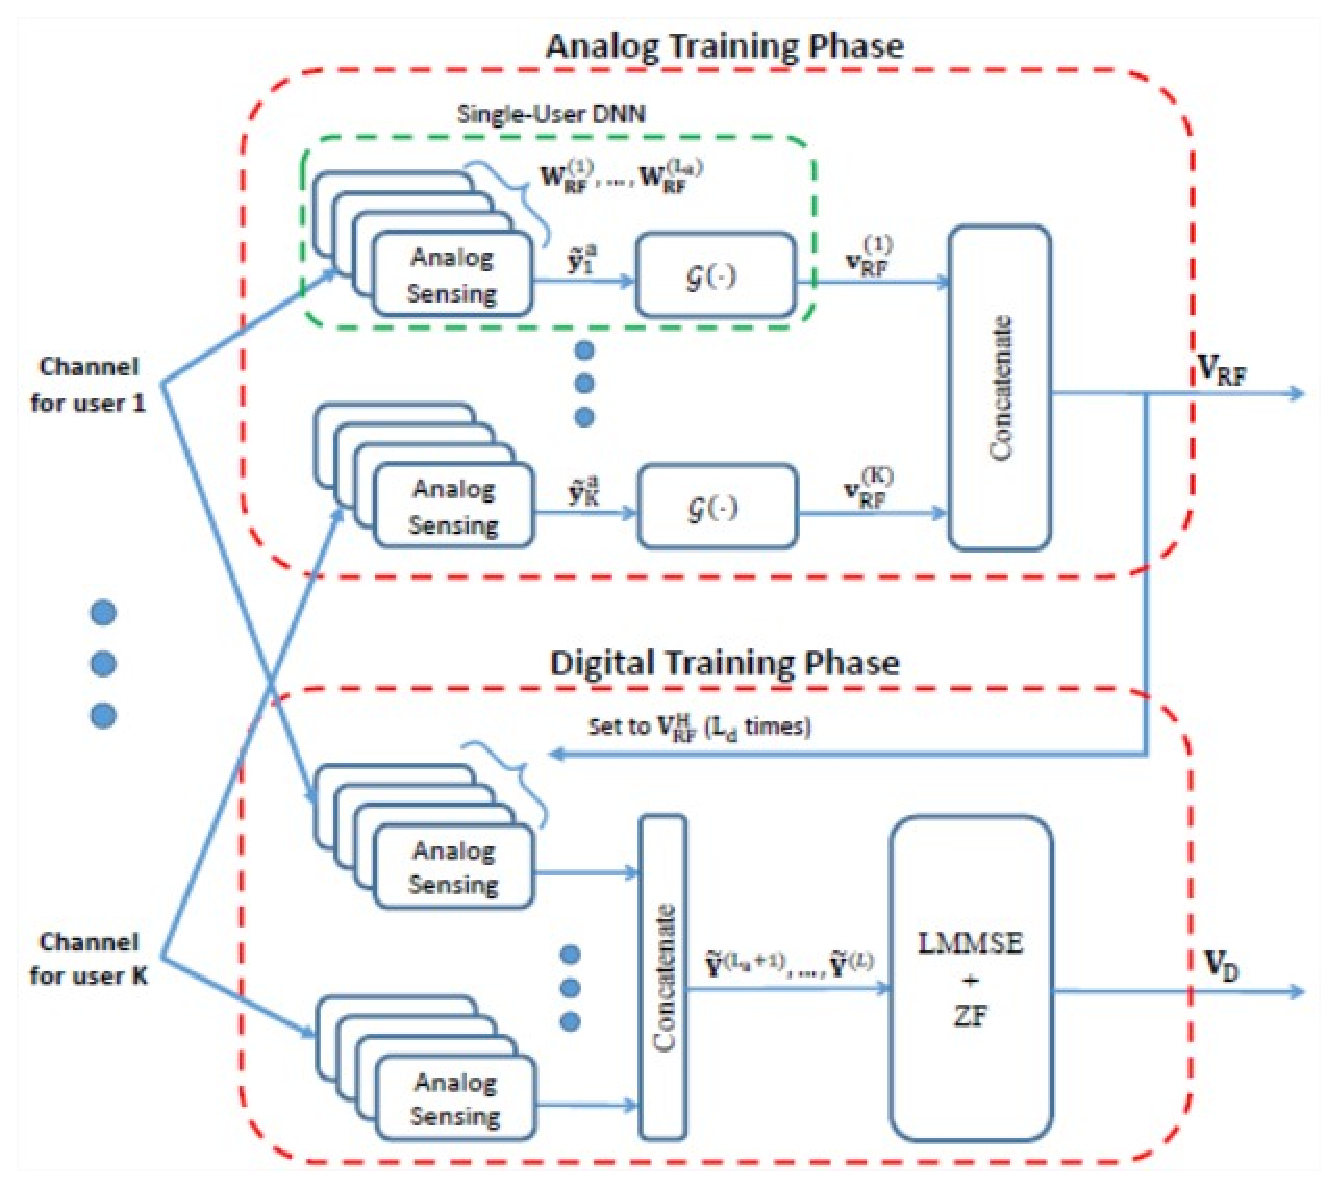
\includegraphics[scale=0.4]{1.eps}
    \caption*{\textit{\small{图}}\small{1}\textit{\small{:设计模拟预编码矩阵和数字预编码矩阵的方法框图}}}
\end{figure}
\vspace{-0.9em}
其中$\gamma_{\mathbf{ZF}}$是确保满足功率约束的标量。 图1说明了提出的方案。

需要注意的是本文提出的体系结构克服了上一节中讨论的限制,特别是:
\begin{itemize}
    \item[$\bullet $]
    本文所提出的方法直接从接收的导频确定混合预编码矩阵,而不必首先估计高维信道。
    \item[$\bullet $]
    与(12)中介绍的直接设计相比,映射矩阵$\mathcal{G}(\cdot)$现在非常容易学习。 
    \item[$\bullet $] 
    单用户DNN的输出维度不是用户数量的函数,因此,该方案可推广到具有任意用户数量的系统。 
\end{itemize}
\vspace{-1.8em}
\subsection{单用户DNN架构}
\vspace{0.2em}
现在我们讨论实现映射$\mathcal{G}(\cdot)$和感知矩阵$\mathbf{W}_{\mathbf{RF}}^{a}$的单用户DNN的细节。具体而言,图2中针对第$k$个用户提
出的体系结构包括传感层,中间层和相位映射层。在DNN的离线训练中,信道和噪声实现$\{\mathbf{h}_{k},\mathbf{n}_{k}\}$被馈送到第一层(即传
感层),并且相应的模拟预编码向量$\mathbf{v}_{\mathbf{RF}}^{(k)}$由最后一层(即相位映射层)产生。 训练后,我们使用$K$个相同的单用户DNN
进行操作,其中在上行链路导频阶段将传感层用作模拟感知矩阵,并将接收到的导频信号$\tilde{\mathbf{y}}_{k}^{a}$馈入中间层以产生下行链路模拟
预编码器。

\textit{1)传感层:}可以将传感矩阵视为DNN的可训练线性层,其中第$k$个用户的信道实现以及噪声作为输入。确实,从(13)中可以看出,$\mathbf{W}_{\mathbf{RF}}^{a}$
只是线性神经网络层中的权重,整体上具有附加的单位模量约束。顺便一提,现有的深度学习库(例如TensorFlow [18])允许创建具有可训练参数的自
定义层。在这种情况下,我们将可训练参数作为感知矩阵$\mathbf{W}_{\mathbf{RF}}^{a}$的相位。
\begin{figure}[H]
    \centering
    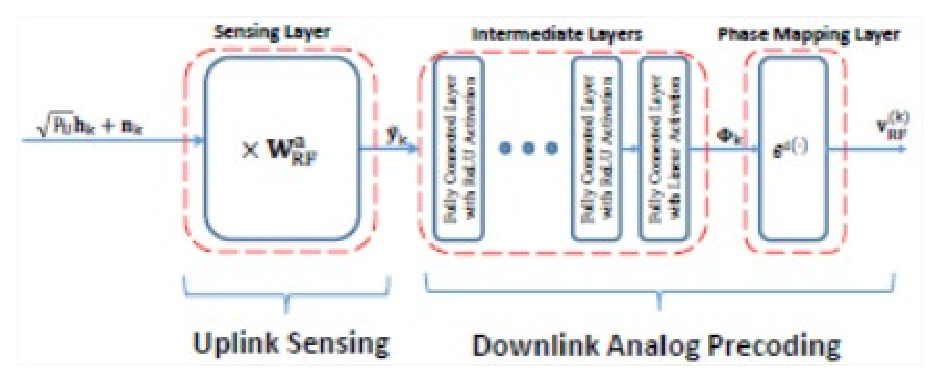
\includegraphics[scale=0.55]{2.eps}
    \caption*{\textit{\small{图}}\small{2}\textit{\small{:用于上行链路感知和下行链路模拟预编码设计的单用户DNN的体系结构}}}
\end{figure}
\vspace{-0.9em}
\textit{2)中间层:}第二级的输入是基带接收的导频矢量$\tilde{\mathbf{y}}_{k}^{a}$,而该级的输出是包含相应模拟预编码矢量的相位的矢量,
用$\Phi_{k}$表示。我们考虑一个包含$R$层组成的中间级,除了最后一层具有线性激活外,其余每一层都与整流线性单元(ReLU)激活完全相连。在数学
上,中间层的输出为:
\begin{align}
\Phi_{k}=\mathbf{W}_{R}\mathscr{R}(.\,.\,.\mathscr{R}(\mathbf{W}_{1}\tilde{\mathbf{y}}_{k}^{a}+\mathbf{b}_{1}).\,.\,.)+\mathbf{b}_{R},
\end{align}
其中$\mathscr{R}(\cdot)=\max(\cdot,0)$是ReLU的激活函数,而$\{\mathbf{W}_{r},\mathbf{b}_{r}\}$是第$r$层的一组可训练参数(即权重和
偏差)。

\textit{3)相位映射层:}该层的输出是用户$k$的模拟预编码向量,因此我们需要强制执行恒模约束。为了实现这一点,我们采用[13]中的思想,
其中(21)的中间层的输出为模拟组合矢量的相位。在这种情况下,该层使用进入式转换$[\mathbf{v}_{\mathbf{RF}}^{(k)}]_{j}=e^{\imath[\Phi_{k}]_{j}}$,
其中$[\cdot]_{j}$表示向量的第$j$个入口。可以使用现有深度学习库中的$Lambda$层来实现这种转换层。

\textit{4)损失函数:}如前所述,第$k$个单用户DNN的损失函数可以近似视为单用户可达到的速率
\begin{align}
\mathscr{L}^{(k)}(\mathbf{h}_{k},\mathbf{v}_{\mathbf{RF}}^{(k)})=-\log_{2}\left(1+\frac{P_{\mathbf{D}}}{MK\sigma^{2}} \left|\mathbf{h}_{k}^{H}\mathbf{v}_{\mathbf{RF}}^{(k)} \right|^{2} \right).
\end{align}
\vspace{-3.0em}
\section{数值结果} 
\vspace{0.2em}
在本节中,我们将本文所提出的混合预编码方法的性能与现有的几种方案进行比较。为此,我们考虑在TDD操作中的单小区大规模MIMO系统,其中BS配备了
均匀的线性阵列,有$M$ = 64根发射天线,且天线之间的距离为半波长。每个用户的信道遵循第II-A节介绍的稀疏信道模型,$L_{p}$= 6,并且路径的
AoDs遵循区间为$[0,2\pi]$的均匀分布。最后,我们将上行链路和下行链路的信噪比设置为$\mathsf{SNR}=10\log P/\sigma^{2}=20\mathsf{dB}$,
其中$P=P_{\mathbf{U}}=P_{\mathbf{D}}$。 在我们的模拟中,我们考虑与以下方案进行比较:

\textit{1)具有完整CSI的混合设计:}该设计遵循文献[10]中的工作,假设该信道是BS完全已知的,并被用作其他方案的基准。在这种设计中,模拟
预编码矩阵是通过匹配信道矩阵的相位获得的(即$[\mathbf{V}_{\mathbf{RF}}]_{ij}=[\mathbf{H}]_{ij}/|[\mathbf{H}]_{ij} | $),
而数字预编码矩阵则是通过对等效信道做ZF算法得到的。
\begin{figure}[H]
    \centering
    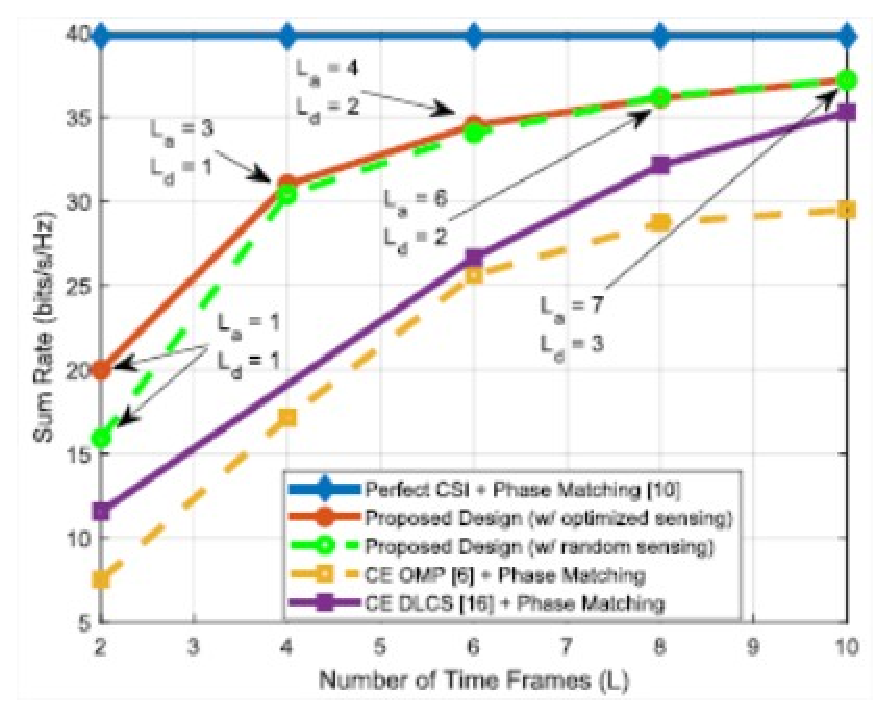
\includegraphics[scale=0.55]{3.eps}
    \caption*{\textit{\small{图}}\small{3}\textit{\small{:当$K=N_{\mathbf{RF}}=4$时,针对不同的L值,本文提出的方法与现有方案的性能比较。}}}
\end{figure}
\vspace{-0.9em}
\textit{2)使用正交匹配追踪(OMP)的具有不完整CSI的混合设计[6]:}在该设计中,使用OMP算法估计每个用户的高维信道的参数,然后使用上述[10]
中的方案从恢复的信道中确定预编码矩阵。

\textit{3)使用深度学习压缩感知(DLCS)的具有不完整CSI的混合设计[16]:}为了克服OMP解析信道路径的复杂方式,[16]的作者开发了一种受OMP启
发的DNN架构来恢复信道参数。我们在这里使用相同的DNN架构来估计信道,并根据[10]中的设计方案从恢复的信道中设计预编码矩阵。

我们使用TensorFlow实现了图2中提出的DNN和DLCS。对于拟议的DNN,我们将中间层的数量设置为$R$= 3,其中密集层的宽度分别为2048、1024和512。
为了更快地收敛,每个密集层之前都有批量规范化层。另外,对于第一层,我们首先按照区间为$[0,2\pi]$的均匀分布来随机设置模拟预编码矩阵的相位。
对于DLCS,我们考虑一个宽度为1024、512、256和128的4层密集网络。对这两个网络的训练是分批进行的,并且需要几个周期。每个批次包含500个样本,
每个周期有20个批次。我们在上行链路训练阶段处理信道和噪声分布,因此我们可以生成训练DNN所需的任意数量的数据样本。

在图3中,对$N_{\mathbf{RF}}=K=4$,我们针对不同的导频帧$L$的数量绘制了总速率。对于所提出的方法,用箭头表示$L_{a}$和$L_{d}$。我们可以看
到,本文提出的方案明显优于OMP和DLCS。例如,与$L = 10$的DLCS相比,本文所提出的方法在L=8时可实现整个CSI系统总和率的90%以上,从而表明与
传统方案相比,导频开销节省了20%以上。这支持了我们的主要观点,即在训练开销有限的混合系统中,信道估计和预编码设计的分离并不是最佳的。
但是我们在这里注意到,在长导频长度的限制下,传统的分离方案可以做得很好。最后,我们观察到,仅在导频长度非常短时,
\begin{figure}[H]
    \centering
    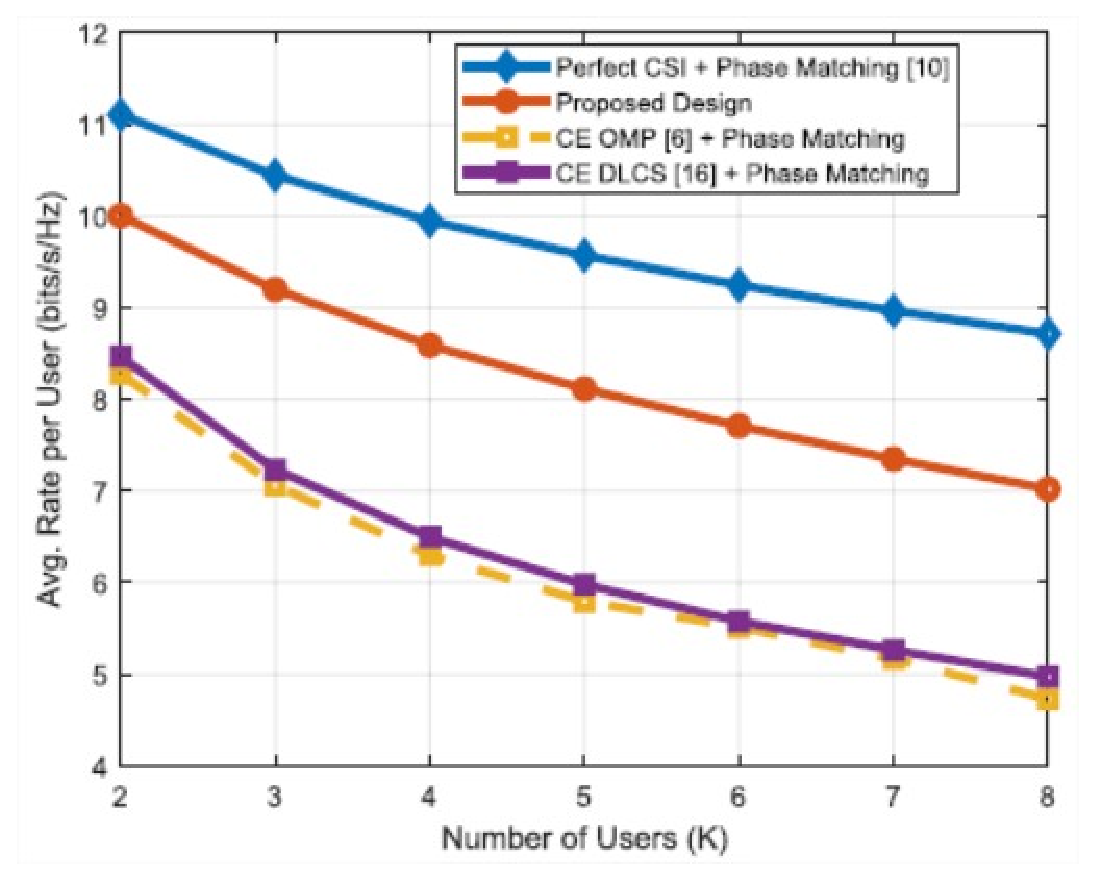
\includegraphics[scale=0.5]{4.eps}
    \caption*{\textit{\small{图}}\small{4}\textit{\small{:该方案对用户数量的普遍性。这里,我们将$N_{\mathbf{RF}}$设为8,$K$从2个用户变到8个用户。}}}
\end{figure}
\vspace{-0.9em}
\noindent 优化信道感知矩阵的效果才显著。

接下来,我们研究关于用户数量的普遍性。为此,我们设$L$= 3,$N_{\mathbf{RF}}$ = 8,并且$K$从2变到8。对于本文的方案,我们设$L_{a} = 2$,
$L_{d} = 1$,并设计了一个用于$K$=8情况的单用户DNN。如果$K$<8,我们做出简化选择,仅使用$K$个$\mathsf{RF}$链进行下行链路预编码。注意,
还必须做出简化选择,以使常规方案能够正常工作。在图4中,我们绘制了所有四种方案的用户平均速率与用户数量之间的关系。我们观察到,与基于信
道恢复的方法相比,我们的方法能够支持有关用户数量的通用操作,同时保持明显更好的性能。
\vspace{-0.4em}
\section{总结}
\vspace{0.7em}
本文介绍了毫米波TDD大规模MIMO系统中模拟预编码和数字预编码矩阵的设计。本文所提出的基于学习的预编码方案可用于任何数量的用户,并且通过直接
从接收到的导频构造预编码矩阵而无需进行估计高维信道的中间步骤克服了现有方案的局限性。数值评估表明,与基于信道恢复的方案相比,频谱效率有了
显着提高。
\bibliographystyle{IEEEtr}
\cite{ref1,ref2,ref3,ref4,ref5,ref6,ref7,ref8,ref9,ref10,ref11,ref12,ref13,ref14,ref15,ref16,ref17,ref18}
\bibliography{refer}
\end{document}


